\chapter{Freddy - \emph{Segmentation}}

Freddy est notre module de segmentation, il utilise OCSFML, et est basé sur l´algorithme RLSA (Run Lenght Smoothing Algorithm).

\section{L'ancienne méthode, ses points faibles}

Au moment de la première soutenance, nous utilisions un algorithme très simple, et moyennement efficace: nous faisions un histogramme horizontal, un tableau de taille la hauteur en pixels de l´image. Nous le remplissions avec le nombre de pixels noirs à la ligne correspondante. Cette opération nous permettait de savoir à quel moment une nouvelle ligne ou un nouveau paragraphe apparaissent.\\
Une fois ce découpage effectué, il nous suffisait de répéter cette opération horizontalement sur chacune des lignes repérées, afin de détecter les mots et caractères composant chacune des lignes.\\
Cependant, nous avons été confrontés à plusieurs problèmes, qui nous ont amenés à chercher une autre méthode plus performante, que nous verrons en détail dans la prochaine section. En effet, avec cette méthode, les caractères avaient tendance à être coupés, ou bien collés à d´autres. Il en était de même pour les lignes, qui avaient tendance à fusionner. Cette technique nécessitait également d´avoir une image sortie du prétraitement parfaite, la moindre impureté ou la moindre ligne, image ruinant totalement le résultat de l´algorithme.

\begin{figure}[h!]
  \centering
  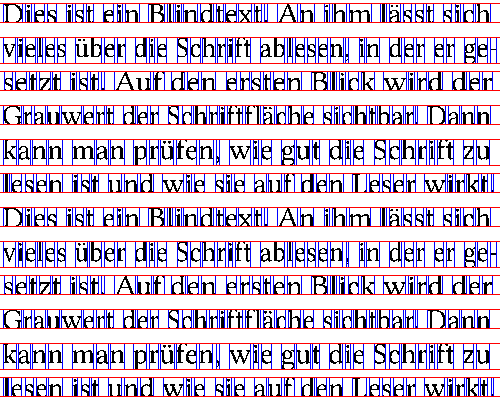
\includegraphics[scale=0.8]{chapters/Pictures/segmented.png}
  \caption{Notre ancien système de segmentation: On peut voir que certains caractères sont collés}
\end{figure}


\section{Le RLSA}

Pour détecter le paragraphes, lignes, mots ou les caractères, nous utilisons donc maintenant l'algorithme Run Lenght Smoothing Algorithm (RLSA) modifié par nos soins, pour couvrir au mieux nos besoins. Le principe est simple: on récupère l´image sortie du prétraitement de lenna. On regarde horizontalement et verticalement quels sont les pixels noirs adjacents, c´est à dire quels sont les pixels noirs séparés de moins de n pixels noirs. Nous allons voir comment définir cette constante, qui n´est évidemment pas ´hardcoded´ dans la partie suivante. Il en résultera donc deux matrices de bouléens aux dimensions de l´image. Dans ces matrices représentant la couleur noire ou blanche des pixels de l´image, nous aurons changé tous les pixels blancs entre deux pixels noirs adjacents. Les images représentées par ces matrices ressemblent à l´image d´entrée, mais comme si l´encre avait bavée horizontalement ou verticalement.\\
Nous appliquons ensuite un opérateur binaire logique entre les bits des deux matrices aux mêmes coordonnées, afin de former une nouvelle matrice. Cette nouvelle matrice, toujours aux dimensions de l´image d´origine, représente l´image résultat, qui sera utilisée pour la suite des traitements. Dans cette image, les lettres, mots, lignes ou paragraphes se retrouveront rassemblés en blocs noirs, suivant le nombre de pixels adjacents que l´on aura considéré.\\
Cette transformation nous permet ensuite, via un autre algorithme que nous détaillerons plus tard, de récupérer les coordonées et dimensions des zones noircies.\\
Ainsi, les images éventuelles n´auront pas plus de valeur qu´un simple caractère, après l´application de cet algorithme, générant très peu d´erreurs lors du passage d´anna, notre réseau de neuronnes.

\begin{center}
  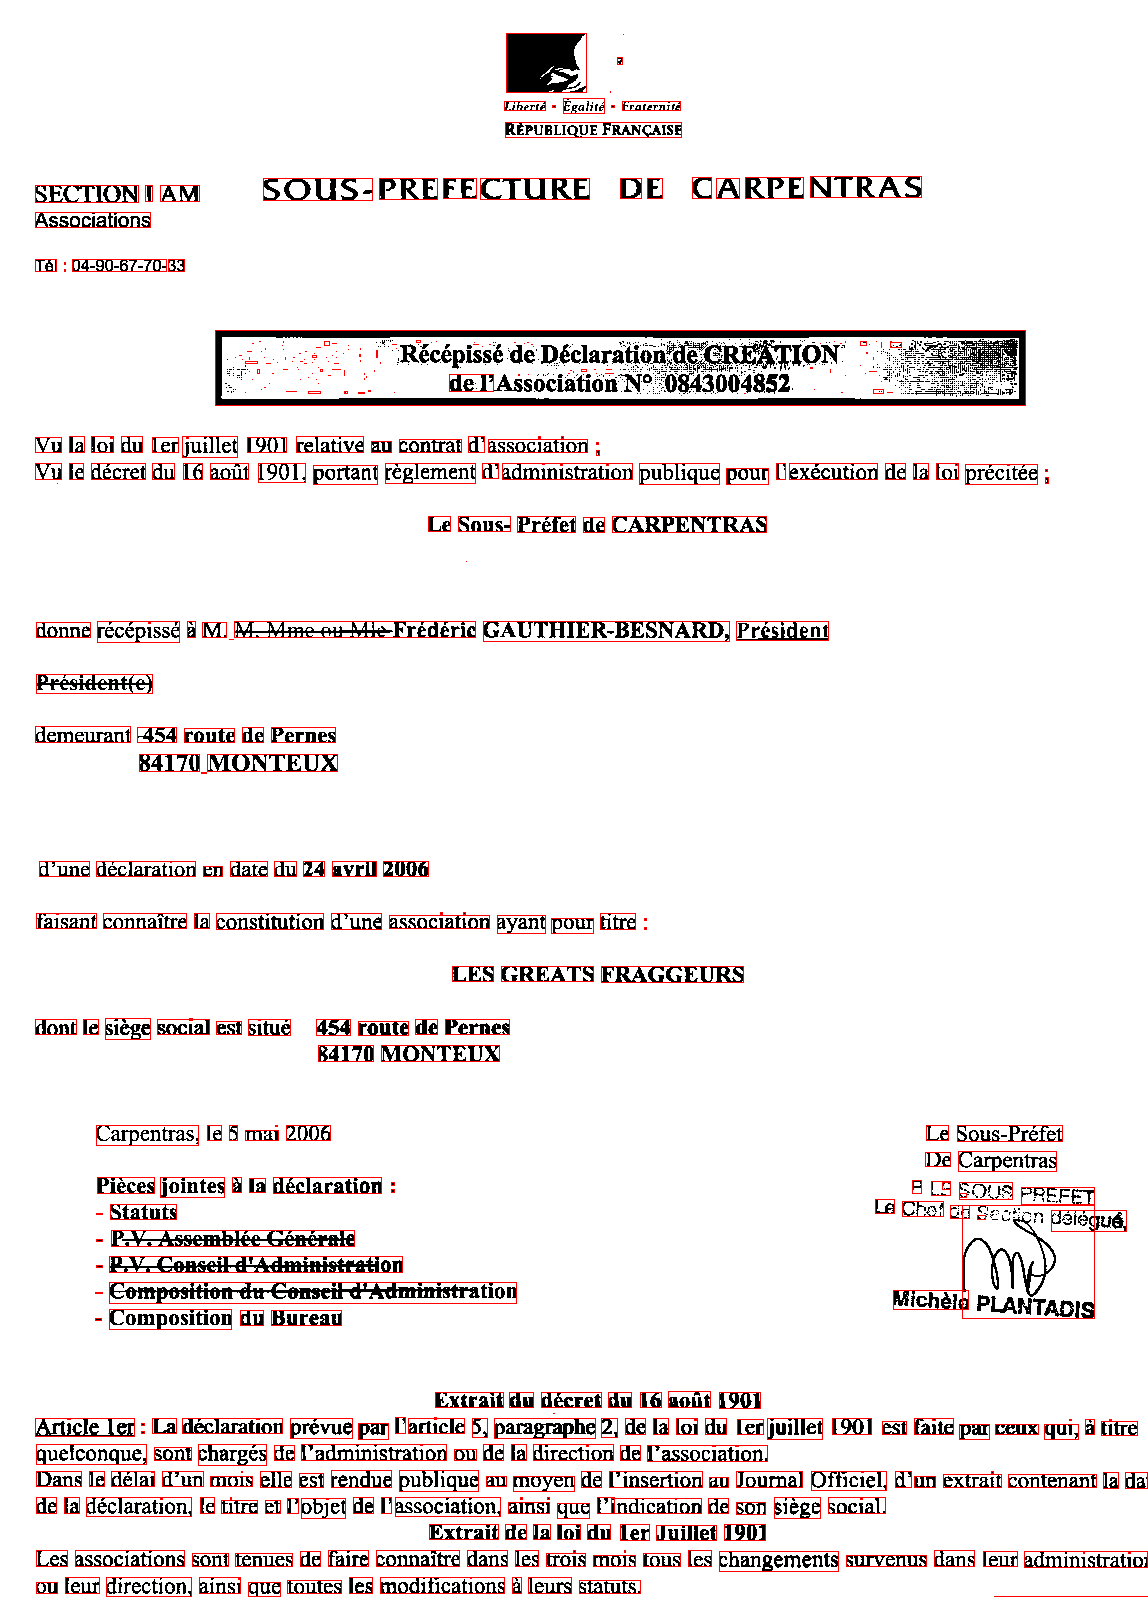
\includegraphics{Pictures/3words.png}
  \caption{Notre algorithme RLSA utilisé pour la détection des mots}
\end{center}

\subsection{La constante d´adjacence}


\subsection{Optimisations}

Pour sélectionner les caractères, mots, lignes ou paragraphes, nous devons modifier la constante représentant le nombre de pixels adjacents à fusionner. Cependant, cette modification seule ne nous permet pas de sélectionner efficacement une partie précise de l´image. En effet, les caractères sont globalement carrés, tandis que les mots et lignes sont assez horizontaux. Une seule constante ne suffira donc plus. Nous utilisons deux constante: une pour la matrice horizontale, et une autre pour la matrice verticale. Nous ne récupérons qu´une seule valeur lors de l´algorithme de la partie précédente. Nous avons cependant pu définir les deux constantes en fonction du retour de la fonction précédente à l´aide de simples multiplications et divisions entières. Il s´est révèlé que ces valeurs fonctionnent très bien pour toutes les images testés jusqu´ici, quelle que soit leur résolution et leur densité de pixels.\\
Contrairement au RLSA classique, nous n´utilisons pas uniquement l´opérateur logique ´et´, mais également le ´ou´. Il se trouve que pour la detection des lignes et des paragraphes, avec plus d´espaces entre les pixels noirs (une proportion de pixels noirs par rapport aux pixels blancs plus faible) que pour les caractères et les mots, le ´ou´ donne de bien meilleurs résultats que le ´et´. Cette méthode également s´est révèlée être très efficace quelle que soit l´image.


\section{Bounding boxes}

Une fois les ´blocs noirs´ formés, il faut récupérer leur coordonnées. Celles-ci sont récupérées sur l´image résultat.\\ %Principe? 
Les bounding boxes seront bien sur utilisées plus tard sur l´image sortie du prétraitement de lenna, sans aucune autre altération. Il n´est pas question de donner à anna une liste de caractères tous complètement noirs.


\subsection{La mise en forme des données}

Toutes les ´bounding boxes´ doivent être mises en ordre, afin d´être utilisables par anna (Nous voulons restituer le texte dans l´ordre, et non les caractères dans un ordre quelconque). En plus de l´ordre, il faut savoir à quel moment un changement de mot, ligne, ou paragraphe a lieu, afin de pouvoir le faire apparaitre sur le document final. La mise en page importe beaucoup. Il est très difficile de lire un texte sans espace entre les mots, ou un minimum de mise en page. C´est encore plus vrai si certaines erreurs apparaissent.\\
Nous avons décidé de représenter les caractères et tous les goupes les contenant (mots, lignes, paragraphes) sous forme de listes imbriquées: nous avons accès à la liste des paragraphes. Les paragraphes sont des listes de lignes, qui sont des listes de mots, qui sont des listes de caractères. Il est facile de parcourir cette structure. A la sortie d´anna, la liste de listes de listes de listes de listes de caractères est transformée en liste de listes de liste de chaînes de caractères. Robert pourra ainsi lire facilement mot par mot.

\begin{figure}[h!]
  \centering
  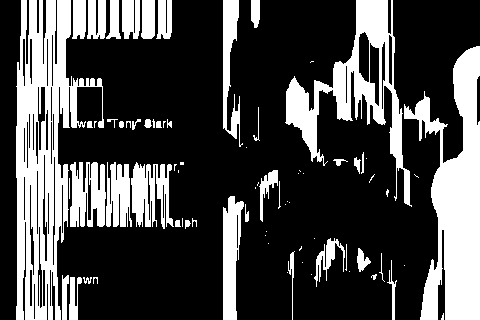
\includegraphics[scale=1]{chapters/Pictures/vrlsa.png}
  \caption{Un exemple de RLSA vertical}
\end{figure}

\begin{center}
\end{center}
